% !TEX root = ../main.tex

\chapter{Otros elementos}
\label{ch:otro}


\section{Figuras y ecuaciones}

Ejemplo de dibujo, véase la figura~\ref{fg:figura}.
\begin{figure}[htb]
\centering	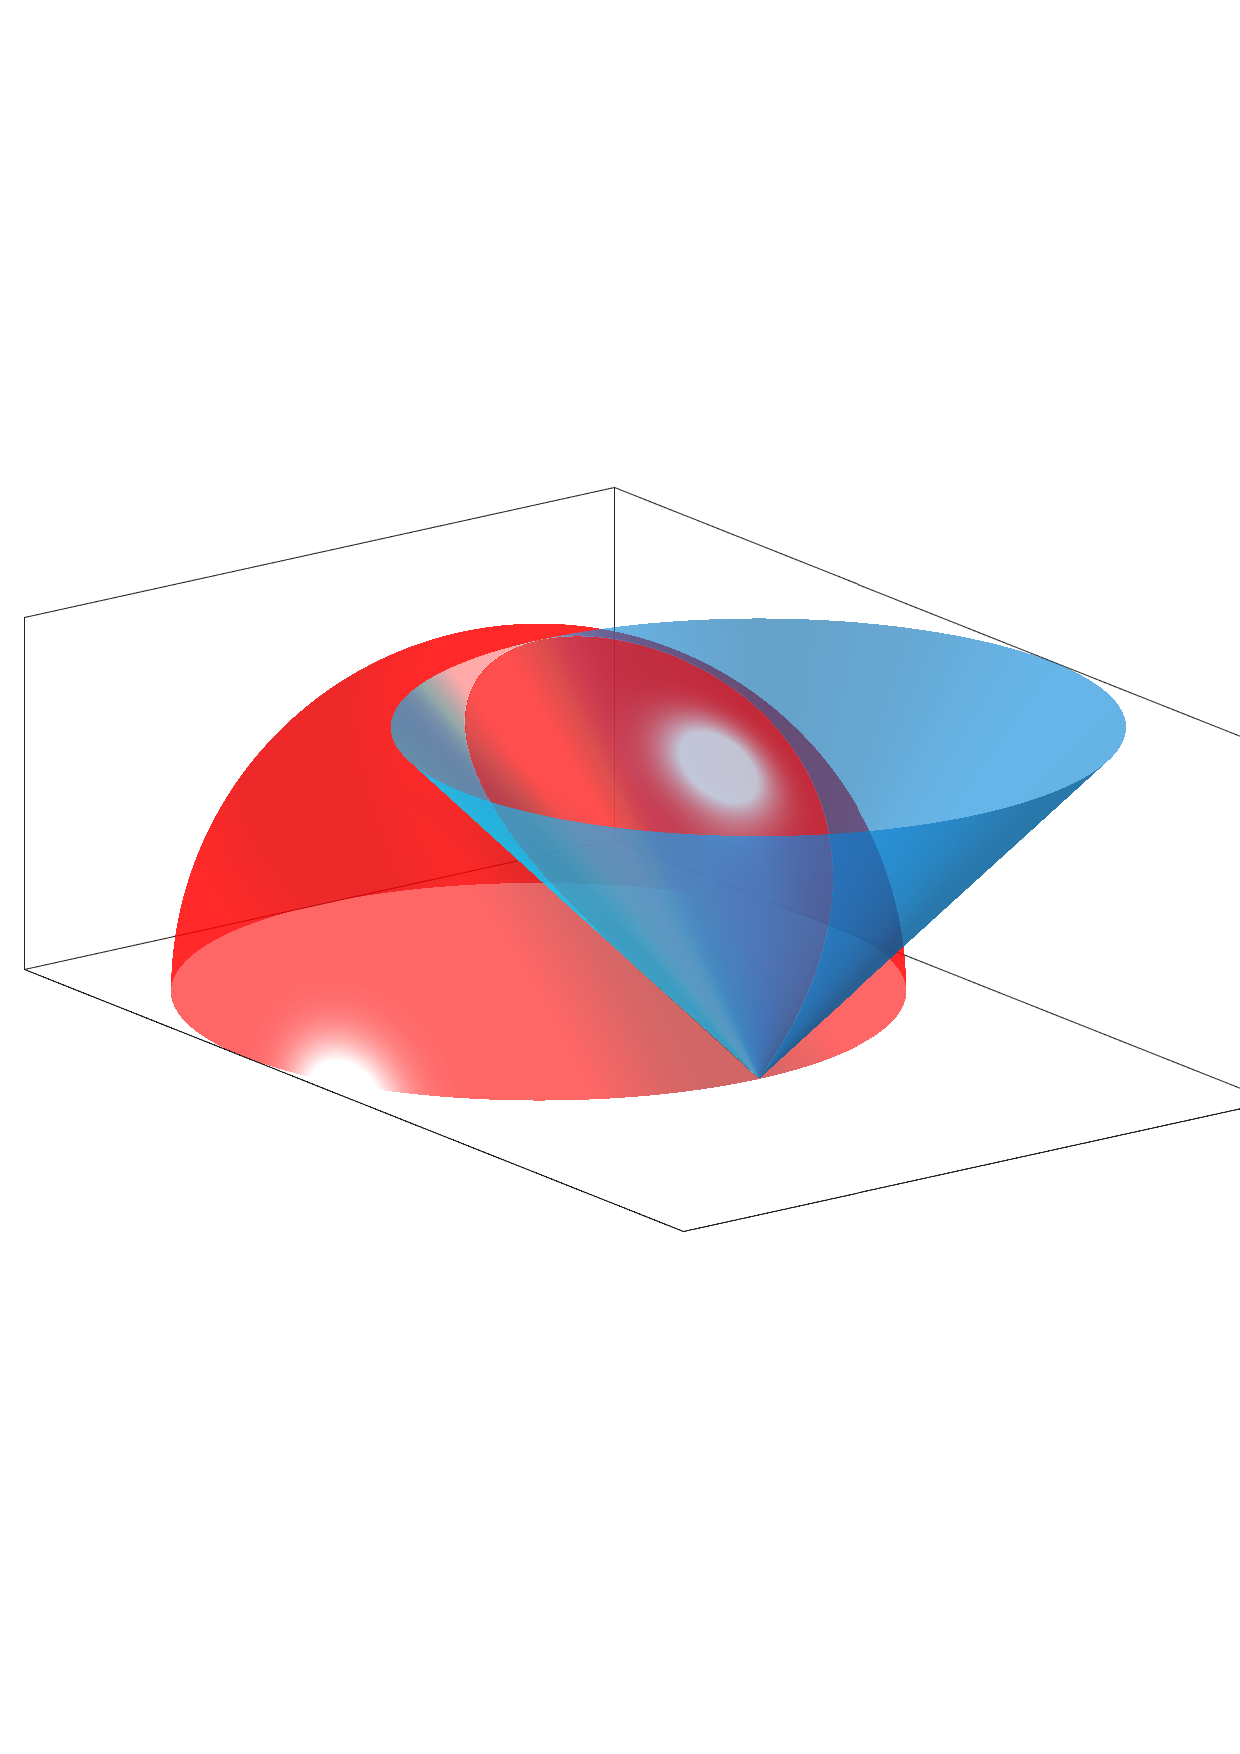
\includegraphics[width=0.5\textwidth]{figures/viviani.pdf}
\caption{Ejemplo de figura.}\label{fg:figura}
\end{figure}

Ejemplo de ecuación. Véase la definición de la función $f$ en~\eqref{fm:formula}.

\begin{equation}\label{fm:formula}
f(x) = \left\{ \begin{array}{ll}
\displaystyle\frac{3}{2}x^2, &  \mbox{si}\; -b \leq x < b; \\[5mm]
\displaystyle\int_{0}^{x} g(t)\, dt,  &  \mbox{resto.}
\end{array}\right.
\end{equation}

\section{Tablas}
Cómo introducir una tabla. Véase la tabla~\ref{tab:mi_etiqueta}.
\begin{table}[ht]
\centering
\begin{tabular}{ccc}
\hline\noalign{\smallskip}
$n$ &$B$ & $S$  \\[1mm]
\hline \noalign{\smallskip}         
 2& $\pi R^2$& $2\pi R$  \\[3mm]
 3& $\displaystyle \frac{4\pi}{3}R^3 $& $4\pi R^2$ \\[3mm]
 \hline \noalign{\smallskip}
\end{tabular}
\caption{Ejemplo de tabla.}
\label{tab:mi_etiqueta}
\end{table}

\section{Definiciones y teoremas}

En la plantilla se han definido entornos para organizar las definiciones y los resultados matemáticos dentro del texto. Estos entornos se hallan en el preámbulo del fichero \verb+main.tex+, para que se puedan modificar si el autor del trabajo prefiere configurarlos de otro modo. A continuación, aparecen algunos ejemplos.
\begin{defn}
    Diremos que un triángulo es \emph{rectángulo}\index{triángulo!rectángulo} si uno de los ángulos es un ángulo recto, esto es, $\tfrac\pi2$. En este triángulo, el lado opuesto al ángulo recto es la \emph{hipotenusa}\index{hipotenusa}, y los otros dos lados se les denomina \emph{catetos}\index{cateto}.

    Cuando en un triángulo, el ángulo de mayor amplitud es mayor que un ángulo recto, diremos que el triángulo es \emph{obtusángulo}\index{triángulo!obtusángulo}; de lo contrario diremos que es \emph{acutángulo}\index{triángulo!acutángulo}.
\end{defn}

\begin{thm}
    En un triángulo rectángulo se cumple la igualdad $a^2=b^2+c^2$, donde $a$ es la longitud de la hipotenusa, y $b$ y $c$ son las longitudes de los catetos.
\end{thm}
\begin{proof}
    Sea $T$ un triángulo rectángulo.
\end{proof}

\begin{rmk}
    La hipotenusa, por definición, es el lado contrario al ángulo recto, pero también coincide con el lado del triángulo de mayor longitud.
\end{rmk}

\begin{exm}
    Las ternas pitagóricas como $(3,4,5)$ son ejemplos de longitudes de los lados de un triángulo rectángulo. En este caso, la longitud de la hipotenusa es~$5$.
\end{exm}

Algunas sugerencias adicionales:
\begin{itemize}
    \item Todas las variables matemáticas deben ir en modo matemático y aparecer en itálicas: ``Sea $X$ el conjunto...''.
    \item En cambio, las funciones comunes como seno, coseno, etc. no deben estar en itálicas: ``Considera la función $f(x)=\sin x$...''.
    \item Evita en lo posible que una ecuación rompa entre dos líneas.
    \item No comiences tus frases con un símbolo (o un número). También eso es deseable para el comienzo de línea.
    \item Destaca una fórmula situándola fuera del texto si al incluirla dentro de la línea de texto normal provoca una separación entre líneas mayor de la diseñada, o cuando se haga referencia a ella en otra parte del texto.
\end{itemize}

Finalmente, se puede usar la letra {\sffamily sin serifa} en el documento para destacar términos.

Las letras griegas más utilizadas son las siguientes:
\[
\alpha,\beta,\gamma,\lambda,\mu
\]